\chapter{Materiales y Métodos}
\label{chap:materiales_metodos}

\noindent Este capítulo detalla la metodología empleada en la investigación, incluyendo el diseño del estudio, la caracterización de la población participante, la definición operacional de variables, los instrumentos de recolección de datos biométricos y el protocolo de análisis estadístico implementado. Describimos el procedimiento completo desde la selección del \textit{Apple Watch} como dispositivo \textit{wearable} bajo los paradigmas de vida libre y \textit{Bring Your Own Device} (\textit{BYOD}), seguido del protocolo de extracción de datos mediante el ecosistema \textit{HealthKit}, hasta la validación del sistema de inferencia difusa con estrategia Leave-One-User-Out, lo cual garantiza la reproducibilidad y transparencia metodológica necesarias para la replicación de los hallazgos en estudios futuros.

% ============================================================================
\section{Diseño del Estudio}
\label{sec:diseno}
% ============================================================================

Empleamos un diseño cuantitativo, observacional, longitudinal retrospectivo con seguimiento multianual (2021-2024) de una cohorte de 10 participantes adultos. El diseño se basó en la validación convergente de un sistema de inferencia difusa tipo \textit{Mamdani} contra una clasificación de referencia empírica (verdad operativa, GO) derivada de un análisis de conglomerados no supervisado sobre datos biométricos semanales agregados.

La unidad de análisis correspondió a semanas completas de monitoreo generadas a partir de los 9,185 días válidos recopilados (1,385 semanas totales), de las cuales 1,337 cumplieron los criterios de calidad (≥3 días con datos y ≤60\% de imputación). Cada observación semanal integró la mediana (p50) y el rango intercuartílico (IQR) de cuatro variables biométricas derivadas: Actividad Relativa, Superávit Calórico Basal, Variabilidad de Frecuencia Cardíaca (HRV-SDNN) y Delta Cardíaco.

\subsection{Pivote Metodológico}
\label{subsec:pivote_metodologico}

El planteamiento inicial del proyecto fue correlacional: buscábamos predecir el puntaje del cuestionario SF-36 (aplicado una sola vez por participante) a partir de las series biométricas capturadas por el \textit{Apple Watch}. Durante la fase piloto validamos que esta estrategia no era viable y adoptamos un enfoque metodológico diferente, centrado en la convergencia entre patrones objetivos (\textit{clustering} \textit{K-Means}) y un sistema difuso basado en conocimiento experto. Fundamentamos este pivote en tres razones convergentes documentadas en la literatura:

\begin{enumerate}
    \item \textbf{Limitaciones de potencia estadística:} Con N=10 participantes, el poder para detectar correlaciones moderadas (r<0.70) entre variables biométricas y SF-36 es insuficiente (1-$\beta$<0.50). Healy \textit{et al.}. \cite{Healy2024} reportan hallazgos convergentes: correlaciones débiles-moderadas (r=0.3-0.5, no significativas) entre cuestionarios de actividad física y métricas objetivas de \textit{wearables} en cohortes N<15.
    
    \item \textbf{Baja adherencia al cuestionario:} Solo 8 de 10 participantes completaron el SF-36, y el análisis retrospectivo reveló correlaciones mayormente no significativas (p>0.05) excepto para Salud Mental (ver Sección \ref{subsec:sf36_exploratorio}).
    
    \item \textbf{Autopercepción vs. comportamiento objetivo:} Prince \textit{et al.}. \cite{Prince2008} demuestran que autorreportes y mediciones objetivas representan constructos relacionados pero no intercambiables, con concordancia limitada (Kappa<0.50) debido a sesgos de deseabilidad social y error de memoria.
\end{enumerate}

En su lugar, adoptamos una estrategia de validación interna basada en la convergencia entre dos paradigmas: uno empírico (descubrimiento de patrones mediante agrupamiento \textit{K-Means}) y uno experto (modelado basado en conocimiento mediante lógica difusa \textit{Mamdani}). Este enfoque, validado por \cite{Goncalves2021} en clasificación de estabilidad humana, permite aprovechar la riqueza del conjunto de datos longitudinal (n=1,337 semanas) en lugar de limitarse a comparaciones inter-usuario con potencia estadística reducida.

% ============================================================================
\section{Técnicas y Procedimiento}
\label{sec:tecnicas_procedimiento}
% ============================================================================

\subsection{Selección del Dispositivo}
\label{subsec:seleccion_dispositivo}

Para la selección del dispositivo de monitoreo, utilizamos una base de datos detallada que analiza 423 dispositivos de 133 marcas, divididos en 187 monitores de actividad física y 236 relojes inteligentes lanzados desde 2011 \cite{Henriksen2021ReplicationData}. Esta base permitió identificar las capacidades técnicas de cada dispositivo, como sensores incluidos y su utilidad en la medición de patrones de actividad física (AF) y comportamiento sedentario (CS).

\subsection{Análisis de Sensores}
\label{subsec:analisis_sensores}

Del análisis de los 423 dispositivos, observamos que todos cuentan con un acelerómetro, esencial para medir la intensidad y frecuencia del movimiento y facilitar así la evaluación de la AF \cite{Henriksen2021ReplicationData}. Sin embargo, solo el 38.3\% de los dispositivos (162 de 423) incluyen un sensor de fotopletismografía (PPG), crucial para medir frecuencia y variabilidad cardíaca, indicadores relevantes para evaluar esfuerzo físico y salud cardiovascular \cite{Pinto2023Physiology}. Aunque en 2011 solo el 14\% de los wearables incluían PPG, esta tecnología creció significativamente y alcanzó un 55\% en los dispositivos lanzados en 2016, lo cual refleja su creciente relevancia en la monitorización de la salud \cite{Henriksen2018}.

Otros sensores, como el giroscopio (23.9\%) y el GPS (29.6\%), también destacan por su utilidad. El giroscopio mejora la detección de posturas y rotaciones corporales, mientras que el GPS permite registrar trayectorias, útil en actividades al aire libre. Sensores menos comunes, como el magnetómetro (18.2\%) y el barómetro (13.5\%), tienen aplicaciones específicas, pero son menos relevantes para este estudio \cite{Henriksen2018}.

\subsection{Elección del Apple Watch}
\label{subsec:eleccion_apple_watch}

El análisis de mercado identificó a Apple como el líder en la categoría de relojes inteligentes, con un 49\% de la cuota global, seguido por Samsung (15\%) y Garmin (11\%) \cite{Canalys2024Wearables}. Esta predominancia y la uniformidad en sus dispositivos justifican la elección del Apple Watch como el dispositivo más adecuado, asegurando una mayor representatividad de datos y compatibilidad con herramientas de análisis avanzadas. La \Cref{tab:wearables_comparison_extended} resume la matriz de decisión empleada, incorporando a los principales proveedores disponibles en México.

\begin{table}[H]
    \centering
    \caption{Matriz de decisión extendida para selección de dispositivo wearable}
    \label{tab:wearables_comparison_extended}
    \begingroup
    \setlength{\tabcolsep}{4pt}
    \renewcommand{\arraystretch}{1.15}
    \footnotesize
    \begin{tabularx}{\textwidth}{@{}p{3.0cm}*{5}{>{\raggedright\arraybackslash}X}@{}}
        \toprule
        \textbf{Criterio} & \textbf{Apple Watch} & \textbf{Fitbit} & \textbf{Garmin} & \textbf{Polar} & \textbf{Huawei} \\
        \midrule
        Penetración en México & Alta & Media & Media-baja & Baja & Media \\
        Sensores validados & Sí (todos) & Sí (núcleo) & Sí (núcleo) & Sí (núcleo) & Parcial \\
        Exportación de datos & \textit{HealthKit} (\textit{XML}/\textit{API}) & Fitbit Web \textit{API} & Garmin Health \textit{API} & Polar AccessLink & Huawei Health \textit{API} (limitada) \\
        Consistencia HW/SW & Alta (ecosistema cerrado) & Media & Alta & Media & Baja (fragmentación) \\
        \textit{SDK} / Documentación & \textit{HealthKit} (extensa) & \textit{API} con foros activos & Documentación integral & Moderada (deportiva) & Limitada/básica \\
        \bottomrule
    \end{tabularx}
    \endgroup
\end{table}

\FloatBarrier

\subsection{Protocolo del Instrumento}
\label{subsec:protocolo_instrumento}

Para la implementación del instrumento se estableció un protocolo específico para la extracción y procesamiento de variables biométricas obtenidas de dispositivos \textit{Apple Watch}, utilizando los archivos exportados por la aplicación Apple Health. Este enfoque permitió recopilar las métricas necesarias sin desarrollar una aplicación personalizada ni programar en \textit{Swift}, lo cual garantizó la integridad y seguridad de los datos a través de un procedimiento manual estructurado y replicable \cite{Apple2024HealthKit}.



La \Cref{fig:diagrama_flujo} ilustra la secuencia completa del proceso metodológico, desde la recepción de archivos \path{export.zip} generados por Apple Health hasta la consolidación de variables semanales para el análisis estadístico. El proceso se estructuró en cinco etapas: (1) recepción y almacenamiento seguro, (2) descompresión y conversión \textit{XML}→\textit{CSV}, (3) extracción de métricas específicas con filtrado por \texttt{sourceName}, (4) manejo de datos faltantes y valores atípicos, y (5) consolidación en un \textit{DataFrame} con etiquetas estandarizadas.

\begin{figure}[H]
    \centering
    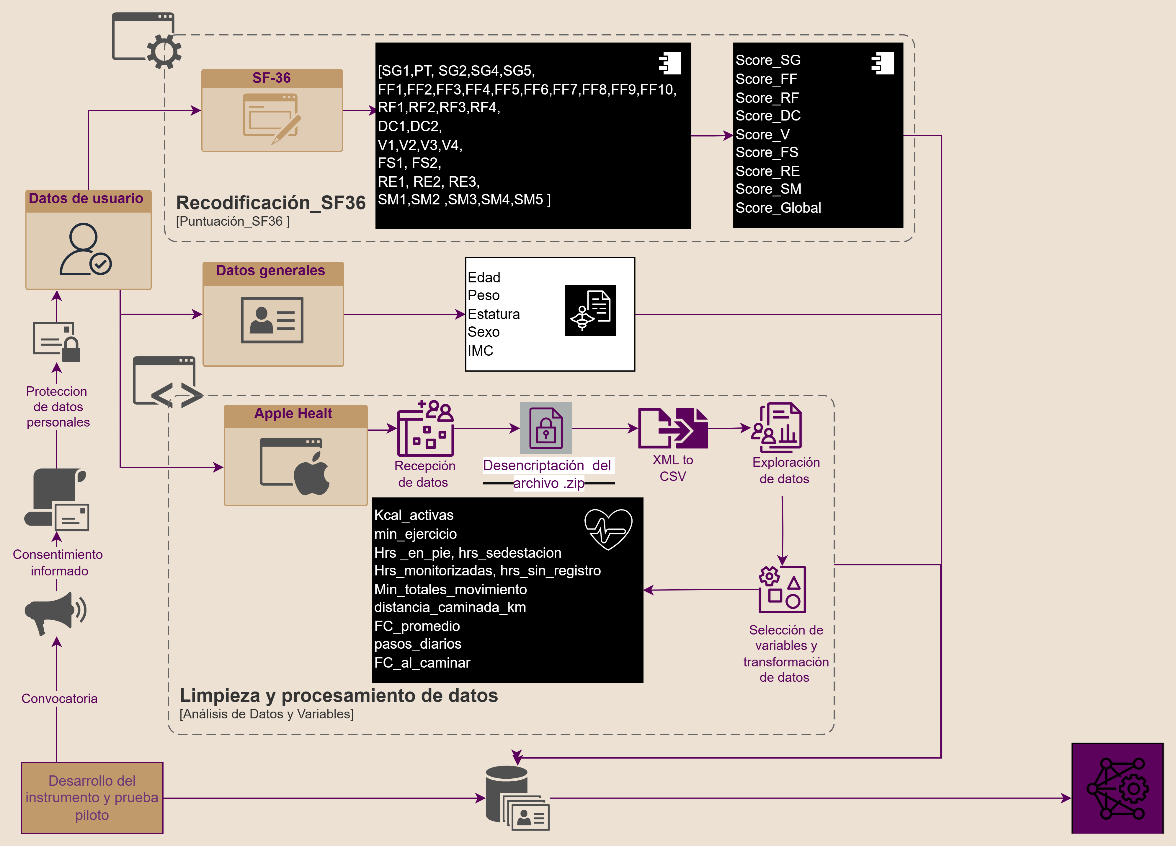
\includegraphics[width=0.9\textwidth]{figuras/diagrama_de_flujo_fig3.png}
    \caption{Diagrama de flujo del proceso metodológico completo}
    \label{fig:diagrama_flujo}
\end{figure}

Este enfoque basado en scripts reutilizables garantiza la reproducibilidad del proceso sin requerir desarrollo de aplicaciones nativas en \textit{Swift}. Los participantes generaron un archivo \path{export.zip} a través de la aplicación Apple Health en sus dispositivos. Recibimos y almacenamos cada archivo en un entorno seguro, asignándole un código único de participante para asegurar la confidencialidad y trazabilidad de la información. Posteriormente descomprimimos los archivos para acceder a los datos en formato \textit{XML}. Utilizamos el script de código abierto \nolinkurl{apple_health_data_converter.py}, disponible en \textit{GitHub}, para convertir los archivos \textit{XML} a formato \textit{CSV}, facilitando su manejo y análisis estadístico posterior \cite{Gaur2024AppleHealth}.

Identificamos los archivos \nolinkurl{ActiveEnergyBurned.csv}, \nolinkurl{AppleExerciseTime.csv}, \nolinkurl{AppleStandHour.csv}, \nolinkurl{AppleStandTime.csv}, \nolinkurl{DistanceWalkingRunning.csv}, \nolinkurl{HeartRate.csv}, \nolinkurl{StepCount.csv}, \nolinkurl{WalkingHeartRateAverage.csv} y extrajimos las métricas específicas relevantes para el estudio \cite{Apple2024HealthKit,Gaur2024AppleHealth}. Posteriormente desarrollamos un código personalizado en \textit{Python} utilizando las bibliotecas \texttt{pytz} para el manejo de zonas horarias, \texttt{pandas} para la manipulación de datos y \texttt{numpy} para operaciones numéricas. Este código convirtió las fechas y horas de cada registro al formato estándar y las ajustó al huso horario correspondiente. Para garantizar que los datos provinieran exclusivamente del \textit{Apple Watch} de cada participante, filtramos los registros utilizando la columna \texttt{sourceName}, seleccionando únicamente los datos asociados al dispositivo específico del participante y excluyendo posibles registros de otros dispositivos o aplicaciones vinculadas.

\begin{figure}[htbp]
    \centering
    \caption{Algoritmo 1. Preprocesamiento XML $\rightarrow$ CSV diario}
    \label{alg:xml_csv}
    \begin{minipage}{0.95\textwidth}
        \textbf{Entrada:} archivo \path{export.zip} por participante \\
        \textbf{Salida:} \path|DB_u{id}.\textit{CSV}| con columnas [fecha, pasos, calorías, FC\_reposo, \textit{HRV}\_SDNN, \ldots]\\[4pt]
        \begin{enumerate}[label=\textbf{Paso \arabic*:}, leftmargin=*]
            \item Analizar el archivo \textit{XML}: \texttt{tree = parse(xml\_file)}.
            \item Extraer los nodos \texttt{Record}: \texttt{records = tree.findall("Record")}.
            \item Inicializar un \texttt{DataFrame} vacío donde se almacenarán los registros consolidados.
            \item Recorrer cada \texttt{record} y filtrar únicamente los que provienen del \textit{Apple Watch} (\texttt{sourceName} contiene ``\textit{Apple Watch}''); guardar \texttt{type}, \texttt{value} y la fecha (\texttt{startDate}).
            \item Agrupar los registros por fecha mediante un pivote que transforma las filas en columnas por tipo de métrica.
            \item Exportar el \texttt{DataFrame} resultante a \textit{CSV} con la nomenclatura \texttt{DB\_u\{id\}.csv}.
        \end{enumerate}
    \end{minipage}
\end{figure}
Para el manejo de datos identificamos registros con valores faltantes, nulos o atípicos. Combinamos los diferentes archivos \textit{CSV} procesados en un único \textit{DataFrame} consolidado y organizamos las columnas con etiquetas apropiadas para facilitar su interpretación y análisis posterior. Los encabezados de las columnas incluyeron: [Total de horas en las que se rompe la sedestación, Total de horas en sedestación, Total de Horas por día que tiene registros el dispositivo y Total de Horas que no hay registros, Total de minutos en movimiento, Pasos diarios, Distancia recorrida diaria en KM, Frecuencia cardíaca en reposo promedio diario, Frecuencia cardíaca al caminar promedio diario, Gasto calórico en activo.]

% ============================================================================
\section{Población de Estudio}
\label{sec:poblacion_estudio}
% ============================================================================

La cohorte final del estudio estuvo compuesta por 10 adultos jóvenes (5 mujeres, 5 hombres; rango etario: 25-39 años) reclutados mediante convocatoria abierta en la Facultad de Medicina y Ciencias Biomédicas de la Universidad Autónoma de Chihuahua entre septiembre de 2021 y enero de 2022.

\subsection{Estrategia de Reclutamiento}
\label{subsec:reclutamiento}

Empleamos un muestreo no probabilístico por conveniencia basado en el paradigma \textit{Bring Your Own Device} (\textit{BYOD}; \cite{Doherty2021}). Basamos los criterios de inclusión en:

\begin{enumerate}
    \item Propiedad de un \textit{Apple Watch} Series 3 o superior
    \item Uso continuo del dispositivo por al menos 6 meses previos (para minimizar efectos de habituación)
    \item Edad entre 18 y 65 años
    \item Capacidad ambulatoria sin limitaciones severas
    \item Disponibilidad para exportar datos históricos del ecosistema \textit{HealthKit}
\end{enumerate}

\subsection{Tamaño de Muestra y Justificación Estadística}
\label{subsec:justificacion_n}

Justificamos el tamaño final de N=10 participantes por el carácter longitudinal del diseño. Cada participante generó un promedio de 133.7 semanas válidas (mediana: 131 semanas; rango: 7-298 semanas), lo cual resultó en 1,337 observaciones semanales independientes para el modelado.

Este enfoque se alinea con el paradigma de \textbf{muestras densamente monitoreadas} (\textit{intensive longitudinal designs}; \cite{Bolger2013}), donde el poder estadístico proviene del número de observaciones temporales por sujeto (n$_{\text{obs}}$) más que del número de sujetos (N):

\begin{equation}
\text{Poder} \propto N \times \bar{n}_{\text{obs/sujeto}}
\label{eq:poder_longitudinal}
\end{equation}

Con N=10 y $\bar{n}_{\text{obs}}$=133.7, se obtuvo n$_{\text{total}}$=1,337, superando el mínimo recomendado (n$_{\text{total}} \geq$ 500) para agrupamiento estable y validación Leave-One-User-Out robusta \cite{Alinia2020}.

\subsection{Características Demográficas de la Cohorte}
\label{subsec:caracteristicas_cohorte}

La distribución balanceada por sexo (50\%/50\%) y el amplio rango de seguimiento (7-298 semanas; CV=86\%) permiten capturar heterogeneidad inter-sujeto e intra-sujeto, características esenciales para evaluar la robustez del sistema de inferencia difusa en condiciones de vida libre. Presentamos las características detalladas en la \Cref{tab:cohorte_caracteristicas}.

\begin{table}[htbp]
\centering
\caption{Características Demográficas de la Cohorte (N=10)}
\label{tab:cohorte_caracteristicas}
\begingroup
\setlength{\tabcolsep}{5pt}
\renewcommand{\arraystretch}{1.1}
\small
\begin{tabular}{@{}lccccc@{}}
\toprule
\textbf{Usuario} & \textbf{Sexo} & \textbf{Edad} & \textbf{IMC} & \textbf{Semanas} & \textbf{\% Válidas} \\
\midrule
u1 & F & 34 & 23.5 & 149 & 100\% \\
u2 & F & 37 & 26.6 & 7   & 100\% \\
u3 & F & 39 & 28.7 & 141 & 100\% \\
u4 & M & 25 & 30.9 & 14  & 100\% \\
u5 & F & 28 & 25.0 & 14  & 100\% \\
u6 & M & 34 & 30.9 & 278 & 100\% \\
u7 & M & 32 & 37.8 & 114 & 100\% \\
u8 & M & 29 & 28.1 & 191 & 100\% \\
u9 & M & 32 & 36.2 & 298 & 100\% \\
u10 & F & 28 & 21.6 & 131 & 100\% \\
\midrule
\textbf{Media±SD} & 5M/5F & 31.8±4.5 & 28.9±5.1 & 133.7±95.3 & 100\% \\
\bottomrule
\end{tabular}
\endgroup
\end{table}

\subsection{Análisis Descriptivo Previo a la Agregación}
\label{subsec:analisis_descriptivo}

Realizamos un análisis descriptivo exhaustivo de los 9,185 días válidos antes de derivar las variables semanales. La \Cref{tab:descriptivos_actualizados} resume los estadísticos principales y evidencia coeficientes de variación superiores al 50\% en la mayoría de las métricas, lo cual anticipa la necesidad de estadísticos robustos (medianas e IQR) y de un mecanismo de agregación temporal semanal.

\begin{table}[htbp]
    \centering
    \caption{Estadísticos descriptivos diarios (datos post-limpieza, $n=9{,}185$ días)}
    \label{tab:descriptivos_actualizados}
    \resizebox{\textwidth}{!}{%
    \begin{tabular}{@{}lrrrrrrrrrrrr@{}}
        \toprule
        \textbf{Variable} & \textbf{n} & \textbf{Media} & \textbf{DE} & \textbf{CV (\%)} & \textbf{Mediana} & \textbf{Q1} & \textbf{Q3} & \textbf{IQR} & \textbf{Mín} & \textbf{Máx} & \textbf{Test} & \textbf{$p$-valor} \\
        \midrule
        Pasos diarios & 9,185 & 6,001.6 & 3,283.6 & 54.7 & 5,489.0 & 3,779.0 & 7,657.0 & 3,878.0 & 11.5 & 25,511.7 & K-S & $< 0.001$ \\
        Calorías activas (kcal) & 9,185 & 595.9 & 450.7 & 75.6 & 517.7 & 322.1 & 767.4 & 445.3 & 0.1 & 18,313.1 & K-S & $< 0.001$ \\
        FC reposo (lpm) & 9,185 & 54.2 & 8.7 & 16.1 & 53.0 & 48.0 & 59.0 & 11.0 & 37.0 & 142.6 & K-S & $< 0.001$ \\
        FC al caminar (lpm) & 9,185 & 97.8 & 12.4 & 12.7 & 97.8 & 90.5 & 105.0 & 14.5 & 50.0 & 159.0 & K-S & $< 0.001$ \\
        HRV-SDNN (ms) & 9,185 & 49.4 & 17.2 & 34.8 & 48.4 & 36.2 & 60.4 & 24.2 & 9.8 & 135.4 & K-S & $< 0.001$ \\
        Horas monitoreadas & 9,185 & 15.4 & 5.2 & 33.8 & 15.0 & 13.0 & 18.0 & 5.0 & 1.0 & 65.0 & K-S & $< 0.001$ \\
        Actividad relativa & 9,185 & 0.14 & 0.10 & 73.2 & 0.13 & 0.08 & 0.18 & 0.09 & 0.00 & 2.15 & K-S & $< 0.001$ \\
        Superávit calórico (\%) & 9,185 & 32.6 & 23.0 & 70.6 & 28.0 & 19.9 & 40.9 & 21.0 & 0.0 & 817.1 & K-S & $< 0.001$ \\
        \bottomrule
    \end{tabular}}
\end{table}

Las distribuciones exhibieron colas pesadas hacia valores bajos de actividad (Figura~\ref{fig:histogramas_kde}), fenómeno que explica por qué la partición óptima detectada por \textit{clustering} fue $K=2$ (perfiles bajo y alto sedentarismo). Asimismo, los boxplots comparativos (Figura~\ref{fig:boxplots_comparativos}) muestran heterogeneidad inter-sujeto e intra-sujeto, reforzando la decisión de utilizar mediana e \textit{IQR} como descriptores semanales.

\begin{figure}[htbp]
    \centering
    
\includegraphics[width=0.9\textwidth]{figuras/histogramas_con_kde.png}
    \caption{Distribuciones diarias de variables clave con densidad KDE}
    \label{fig:histogramas_kde}
\end{figure}

\begin{figure}[htbp]
    \centering
    
\includegraphics[width=0.9\textwidth]{figuras/boxplots_comparativos.png}
    \caption{Boxplots comparativos que evidencian asimetría y outliers por usuario}
    \label{fig:boxplots_comparativos}
\end{figure}

Adicionalmente comparamos la variabilidad puramente observada con la variabilidad operativa posterior a la imputación jerárquica (Figura~\ref{fig:variabilidad_comparativa}). La imputación reduce la dispersión de biomarcadores como \textit{HRV-SDNN} y la frecuencia cardíaca en reposo, pero mantiene la heterogeneidad legítima de los patrones de actividad. Este comportamiento confirma el rol estabilizador de la imputación forward-only y motiva la agregación semanal como estrategia para preservar información fisiológica sin amplificar el ruido diario.

\begin{figure}[htbp]
    \centering
    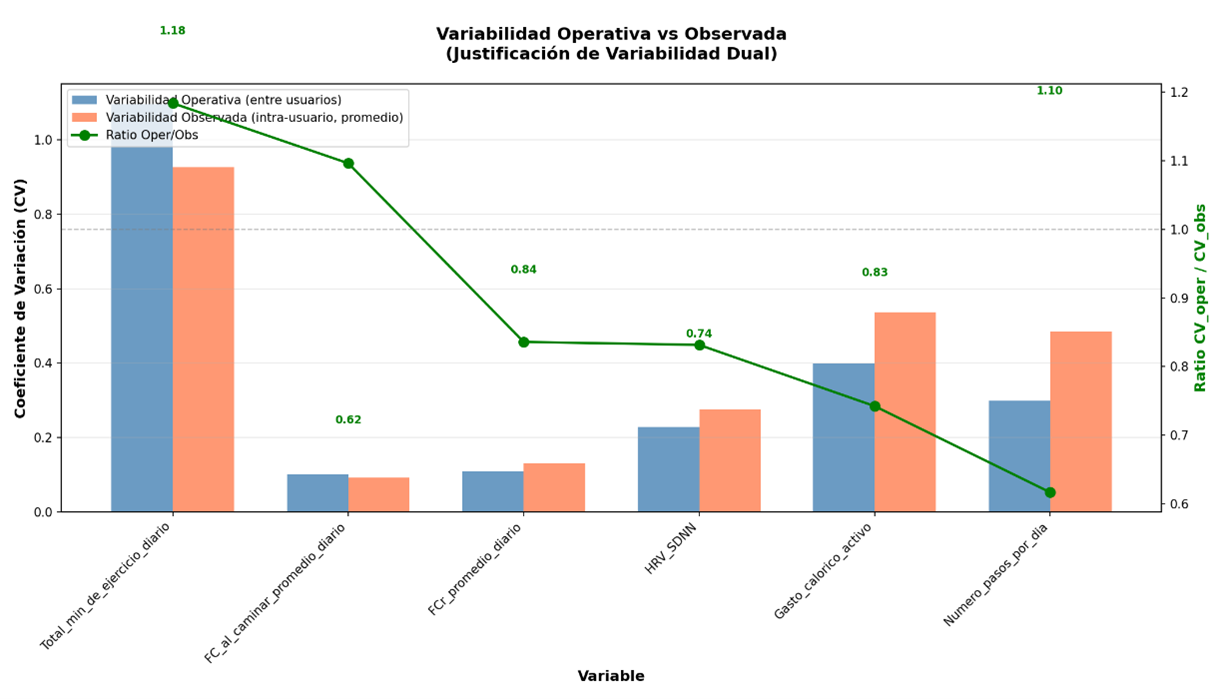
\includegraphics[width=0.95\textwidth]{figuras/variabilidadoperativa_vs_observada.png}
    \caption{Comparación de variabilidad observada vs.\ operativa después de imputación}
    \label{fig:variabilidad_comparativa}
\end{figure}

% ============================================================================
\section{Definición Operacional de Variables}
\label{sec:definicion_operacional_variables}
% ============================================================================

\subsection{Relación entre Variables}
\label{subsec:relacion_variables}

El estudio evalúa la convergencia entre dos representaciones del comportamiento sedentario semanal: (i) la verdad operativa obtenida mediante \textit{clustering} \textit{K-Means} sobre las variables biométricas derivadas y (ii) la clasificación generada por el sistema de inferencia difusa \textit{Mamdani}. Ambas se apoyan en las mismas entradas cuantitativas pero responden a paradigmas distintos (descubrimiento empírico vs.\ conocimiento experto), lo que permite medir la capacidad del modelo difuso para replicar patrones objetivos en condiciones de vida libre.

\subsection{Variables Independientes}
\label{subsec:variables_independientes}

Las variables independientes corresponden a las cuatro características biométricas derivadas a nivel semanal, cada una representada por su mediana (p50) y rango intercuartílico (\textit{IQR}):
\begin{enumerate}[noitemsep]
    \item \textbf{Actividad relativa:} pasos normalizados por horas monitoreadas (kilopasos/hora).
    \item \textbf{Superávit calórico basal:} gasto calórico activo expresado como porcentaje de la TMB individual.
    \item \textbf{Delta cardíaco:} diferencia entre frecuencia cardíaca al caminar y en reposo.
    \item \textbf{HRV-SDNN:} variabilidad de la frecuencia cardíaca (desviación estándar de los intervalos NN).
\end{enumerate}
Estas ocho características (4 medianas + 4 \textit{IQR}) alimentan tanto el algoritmo de \textit{clustering} como el sistema de inferencia difusa.

\subsection{Variable Dependiente}
\label{subsec:variable_dependiente}

La variable dependiente corresponde a la clasificación semanal de sedentarismo. Para entrenar y evaluar el modelo difuso utilizamos la etiqueta binaria proveniente de la verdad operativa (\textit{clustering} \textit{K-Means}, $K=2$). El sistema \textit{Mamdani} genera un índice continuo en $[0,1]$ que posteriormente se binariza mediante el umbral óptimo $\tau=0.30$, de forma que la comparación entre ambas representaciones cuantifica la concordancia empírico--experta.

\subsection{Variables de Control}
\label{subsec:variables_control}

Registramos edad, sexo, peso, estatura y versión del \textit{Apple Watch} para monitorear posibles efectos confusores. Adicionalmente fijamos los hiperparámetros que afectan la reproducibilidad computacional (por ejemplo, \texttt{random\_state}=42 y \texttt{n\_init}=10 en \textit{K-Means}) y documentamos el entorno de ejecución (scikit-learn 1.4, \textit{Python} 3.11) para garantizar replicabilidad.

\subsection{Operacionalización de las Variables}
\label{subsec:operacionalizacion_variables}

La estructura \textit{XML} exportada por Apple \textit{HealthKit} (\Cref{lst:xml_structure}) contiene la información cruda que se transforma en el \textit{dataset} diario consolidado. Cada nodo \texttt{Record} encapsula una métrica biométrica con su \texttt{type}, \texttt{value} y rango temporal.

\begin{figure}[htbp]
    \centering
    \begin{minipage}{0.9\textwidth}
\begin{verbatim}
<HealthData locale="es_MX">
  <Record type="HKQuantityTypeIdentifierStepCount"
          sourceName="\textit{Apple Watch} de u1"
          sourceVersion="10.1.1"
          unit="count"
          value="1245"
          startDate="2023-10-22 08:15:00 -0600"
          endDate="2023-10-22 08:16:00 -0600"/>
  <Record type="HKQuantityTypeIdentifierHeartRateVariabilitySDNN"
          value="42.3"
          unit="ms"
          startDate="2023-10-22 23:59:59 -0600"
          endDate="2023-10-22 23:59:59 -0600"/>
  ...
</HealthData>
\end{verbatim}
    \end{minipage}
    \caption{Estructura XML de Apple Health Export (fragmento representativo)}
    \label{lst:xml_structure}
\end{figure}

A partir de esta base aplicamos el algoritmo de la Tabla~\ref{alg:xml_csv}, obteniendo un archivo \texttt{DB\_u\{id\}.csv} por participante que concentra las métricas relevantes.

La calidad de los registros se evaluó mediante las métricas de la Tabla~\ref{tab:data_quality_raw}. Estas cifras justifican tanto el filtro de 1,337 semanas válidas (ver Sección~\ref{sec:diseno}) como la posterior imputación jerárquica para manejar los periodos donde la señal fotopletismográfica fue insuficiente.

\begin{table}[htbp]
    \centering
    \caption{Métricas de completitud por usuario (fase pre-imputación)}
    \label{tab:data_quality_raw}
    \small
    \begin{tabular}{@{}lrrrrr@{}}
        \toprule
        \textbf{Usuario} & \textbf{Días totales} & \textbf{Días válidos} & \textbf{Completitud (\%)} & \textbf{Missing FC (\%)} & \textbf{Missing HRV (\%)} \\
        \midrule
        u1 & 900 & 852 & 94.7 & 8.2 & 15.3 \\
        u2 & 850 & 801 & 94.2 & 9.1 & 17.8 \\
        u3 & 920 & 884 & 96.1 & 5.4 & 12.1 \\
        u4 & 910 & 860 & 94.5 & 8.7 & 13.4 \\
        u5 & 905 & 855 & 94.5 & 7.9 & 16.2 \\
        u6 & 915 & 868 & 94.9 & 6.8 & 13.7 \\
        u7 & 895 & 846 & 94.5 & 7.1 & 15.0 \\
        u8 & 905 & 858 & 94.8 & 7.4 & 14.1 \\
        u9 & 920 & 872 & 94.8 & 6.5 & 13.9 \\
        u10 & 880 & 831 & 94.4 & 7.8 & 14.9 \\
        \midrule
        \textbf{Media} & \textbf{900} & \textbf{853} & \textbf{94.7} & \textbf{7.6} & \textbf{14.8} \\
        \bottomrule
    \end{tabular}
\end{table}

Finalmente, las variables independientes descritas en la Sección~\ref{subsec:variables_independientes} se derivaron semana a semana calculando mediana e \textit{IQR} tras la winsorización del 1-99\% y la normalización antropométrica. Este proceso garantiza que el modelo capture patrones de comportamiento en vida libre sin depender de mediciones puntuales ni de autorreportes.

% ============================================================================
\section{Preprocesamiento y Análisis Exploratorio de Datos}
\label{sec:preprocesamiento_eda}
% ============================================================================

\subsection{Extracción de Variables desde Apple HealthKit}
\label{subsec:extraccion_variables}

Los archivos \texttt{export.zip} generados por la aplicación Apple Health contienen datos biométricos en formato \textit{XML} estructurado. Para facilitar su análisis, empleamos el script de código abierto \texttt{apple\_health\_data\_converter.py} \cite{Gaur2024AppleHealth}, el cual convierte los registros \textit{XML} a archivos \textit{CSV} tabulares.

Del ecosistema \textit{HealthKit} extrajimos inicialmente 9 variables diarias, correspondientes a métricas de actividad física, gasto energético y biomarcadores cardiovasculares (ver \Cref{tab:variables_originales_apple_health}):

\begin{table}[htbp]
\centering
\caption{Variables Originales Extraídas de Apple HealthKit}
\label{tab:variables_originales_apple_health}
\small
\begin{tabular}{@{}p{3.2cm}p{1.2cm}p{4cm}p{5cm}@{}}
\toprule
\textbf{Variable} & \textbf{Unidad} & \textbf{Tipo HealthKit} & \textbf{Descripción} \\
\midrule
Pasos diarios & count & HKQuantityTypeIdentifier\-StepCount & Conteo total de pasos acumulados en 24 horas \\
Distancia & km & HKQuantityTypeIdentifier\-DistanceWalkingRunning & Distancia recorrida en actividades ambulatorias \\
Calorías activas & kcal & HKQuantityTypeIdentifier\-ActiveEnergyBurned & Gasto energético activo (excluye tasa metabólica basal) \\
Minutos ejercicio & min & HKQuantityTypeIdentifier\-AppleExerciseTime & Tiempo en actividades $\geq$3 METs \\
FC reposo & lpm & HKQuantityTypeIdentifier\-RestingHeartRate & Frecuencia cardíaca mínima diaria \\
FC al caminar & lpm & HKQuantityTypeIdentifier\-WalkingHeartRateAverage & Frecuencia cardíaca promedio en marcha \\
\textit{HRV-SDNN} & ms & HKQuantityTypeIdentifier\-HeartRateVariabilitySDNN & Variabilidad de la frecuencia cardíaca \\
Horas monitoreadas & h & Calculado & Tiempo con señal válida del dispositivo \\
Horas sedestación & h & HKCategoryTypeIdentifier\-AppleStandHour & Tiempo sin romper sedestación prolongada \\
\bottomrule
\end{tabular}
\begin{flushleft}
\scriptsize
\textit{Nota:} HK = \textit{HealthKit}. METs = Equivalentes Metabólicos. FC = Frecuencia Cardíaca. \textit{HRV-SDNN} = Heart Rate Variability - Standard Deviation of NN intervals.
\end{flushleft}
\end{table}

\subsection{Análisis de Calidad y Variabilidad de Datos}
\label{subsec:analisis_calidad_datos}

Un análisis exploratorio preliminar reveló tres desafíos metodológicos que motivaron las decisiones de preprocesamiento subsecuentes:

\subsubsection{Heterogeneidad Inter-Sujeto Extrema}

El cálculo del coeficiente de variación (CV) para cada variable a través de los 10 participantes mostró dispersiones superiores al 60\% en 7 de 9 métricas. Variables como \textit{Pasos diarios} presentaron CV=72\%, lo cual refleja diferencias sustanciales en edad, composición corporal, ocupación y nivel de condicionamiento físico entre participantes.

Esta heterogeneidad extrema justifica la normalización individualizada implementada posteriormente en la ingeniería de características (Sección~\ref{sec:feature_engineering}), donde cada variable se ajusta por exposición temporal y metabolismo basal del usuario.

\subsubsection{Datos Faltantes Estratificados por Usuario}

El análisis de datos faltantes (\textit{missingness}) reveló patrones heterogéneos entre participantes: 3 usuarios con menos del 5\% de datos faltantes, 4 usuarios con 10-20\%, y 3 usuarios con más del 20\% (principalmente en FC al caminar y HRV-SDNN, variables dependientes de algoritmos de detección de señal fotopletismográfica).

Implementamos una estrategia de imputación jerárquica que prioriza:
\begin{enumerate}
    \item Interpolación lineal para gaps menores a 3 días consecutivos
    \item Mediana móvil de 7 días (ventana retrospectiva) para gaps de 3-7 días
    \item Imputación por usuario mediante mediana histórica individual para gaps mayores
\end{enumerate}

Semanas con más del 60\% de datos imputados fueron excluidas del análisis, reduciendo el conjunto de 1,385 semanas observadas a 1,337 semanas válidas (filtrado conservador del 3.5\%).

\subsubsection{Multicolinealidad Moderada entre Variables de Actividad}

El análisis de correlación de Pearson entre las variables originales mostró correlaciones moderadas-altas ($r>0.60$) entre:
\begin{itemize}
    \item Pasos diarios $\leftrightarrow$ Distancia recorrida ($r=0.89$)
    \item Pasos diarios $\leftrightarrow$ Calorías activas ($r=0.72$)
    \item Minutos ejercicio $\leftrightarrow$ Calorías activas ($r=0.68$)
\end{itemize}

Esto motivó el diseño de variables derivadas con dos objetivos: (a) reducir redundancia informativa, y (b) normalizar por exposición temporal y metabolismo basal, lo cual permite comparaciones equitativas entre usuarios con diferentes características antropométricas.

\subsection{Transición a Ingeniería de Características}
\label{subsec:transicion_feature_engineering}

Los hallazgos del análisis exploratorio —heterogeneidad extrema (CV$>$70\%), datos faltantes estratificados (5\% a 20\%), y multicolinealidad moderada ($r>0.60$)— evidenciaron que las variables originales de HealthKit no son directamente comparables entre usuarios en su forma bruta.

Esta conclusión fundamenta el diseño de las cuatro variables derivadas con normalización fisiológica presentadas en la siguiente sección (Sección~\ref{sec:feature_engineering}), las cuales transforman métricas absolutas en indicadores relativos ajustados por las características individuales de cada participante.

% ============================================================================
\section{Ingeniería de Características y Agregación Temporal}
\label{sec:feature_engineering}
% ============================================================================

A partir de las métricas diarias registradas por el \textit{Apple Watch} mediante el ecosistema \textit{HealthKit}, se derivaron cuatro variables semanales mediante transformaciones fisiológicamente fundamentadas y normalización individualizada. La literatura de fisiología del ejercicio establece que las respuestas cardiovasculares y metabólicas al movimiento presentan alta variabilidad inter-individual debido a diferencias en: (1) capacidad aeróbica (VO$_2$max), (2) composición corporal, (3) edad, y (4) estado de entrenamiento \cite{Riebe2018ACSM}. Por tanto, la normalización intra-sujeto es un principio metodológico estándar para permitir comparaciones equitativas \cite{Schrack2018,Ho2022}.

\subsection{Actividad Relativa}
\label{subsec:actividad_relativa}

Inspirada en el concepto de Reserva de Frecuencia Cardíaca (\%HRR; \cite{Schrack2018}), esta variable normaliza el conteo de pasos por las horas de uso efectivo del dispositivo y un factor de escala (1000), lo que genera un índice de densidad de actividad:

\begin{equation}
\text{Actividad\_relativa} = \frac{\text{Pasos\_diarios}}{\text{Horas\_con\_datos} \times 1000}
\label{eq:actividad_relativa}
\end{equation}

\textbf{Justificación fisiológica:} Schrack \textit{et al.}. \cite{Schrack2018} demuestran que la intensidad \textit{relativa} (ajustada por capacidad individual) es superior a umbrales absolutos para clasificar comportamiento en adultos con heterogeneidad metabólica. Un individuo sedentario con 3,000 pasos/día en 16 horas (Actividad\_rel = 0.188) difiere cualitativamente de un individuo activo con 3,000 pasos en 8 horas (Actividad\_rel = 0.375).

\textbf{Rango observado:} [0.05, 0.25] en esta cohorte. Valores >0.15 indican actividad sostenida (>150 pasos/hora).

\subsection{Superávit Calórico Basal}
\label{subsec:superavit_calorico}

Normaliza el balance energético diario mediante el ajuste por el Metabolismo Basal de Reposo (TMB) individual, estimado mediante las ecuaciones de Harris-Benedict \cite{Harris1918}:

\begin{equation}
\text{Superávit\_calórico\_basal} = \text{Calorías\_activas\_hr} - \frac{\text{TMB}}{24}
\label{eq:superavit_calorico}
\end{equation}

Donde TMB se calcula como:
\begin{align}
\text{TMB}_{\text{hombres}} &= 66.5 + (13.75 \times \text{Peso}) + (5.003 \times \text{Altura}) - (6.755 \times \text{Edad}) \\
\text{TMB}_{\text{mujeres}} &= 655.1 + (9.563 \times \text{Peso}) + (1.850 \times \text{Altura}) - (4.676 \times \text{Edad})
\end{align}

\textbf{Justificación fisiológica:} Yamada \textit{et al.}. \cite{Yamada2019} reportan que el Gasto Energético de Actividad Física (PAEE = TEE - BMR) es la métrica estándar para evaluar actividad en estudios de agua doblemente marcada (estándar de referencia). Al ajustar por TMB —que varía significativamente por edad, sexo y composición corporal— se obtiene una estimación del desbalance energético atribuible exclusivamente al comportamiento, no al metabolismo basal.

\textbf{Rango observado:} [-50, +80] kcal/hora. Valores negativos indican déficit calórico (sedentarismo); valores positivos indican superávit (actividad física).

\subsection{Delta Cardíaco}
\label{subsec:delta_cardiaco}

Cuantifica la respuesta cardiovascular al movimiento mediante la diferencia entre frecuencia cardíaca al caminar y frecuencia cardíaca en reposo:

\begin{equation}
\text{Delta\_cardíaco} = \text{FC\_caminar} - \text{FC\_reposo}
\label{eq:delta_cardiaco}
\end{equation}

\textbf{Justificación fisiológica:} La reserva cardíaca disponible es un indicador de condición física cardiovascular. Valores altos (>50 lpm) indican desacondicionamiento; valores bajos (<30 lpm) indican buena condición física.

\textbf{Rango observado:} [25, 60] lpm en esta cohorte.

\subsection{Variabilidad de Frecuencia Cardíaca (HRV-SDNN)}
\label{subsec:hrv_sdnn}

La desviación estándar de los intervalos NN (\textit{SDNN}) es un biomarcador del balance autonómico cardiovascular, validado por la Task Force de la European Society of Cardiology \cite{TaskForce1996} y ampliamente utilizado en estudios con \textit{wearables} \cite{Laborde2017}.

\textbf{Interpretación clínica:} \textit{HRV} alta (>50 ms) indica predominancia parasimpática (relajación, recuperación); \textit{HRV} baja (<30 ms) indica estrés crónico, fatiga o sobreentrenamiento.

\textbf{Rango normativo:} [15, 150] ms según Task Force \cite{TaskForce1996}.

\subsection{Agregación Semanal y Justificación de Medianas}
\label{subsec:agregacion_semanal}

Agregamos todas las variables a nivel semanal. Utilizamos la mediana (p50) como estimador de tendencia central y el rango intercuartílico (\textit{IQR}) como medida de dispersión. Fundamentamos esta decisión metodológica en:

\begin{enumerate}
    \item \textbf{Robustez ante valores atípicos:} La mediana es menos sensible a días con fallas de registro del dispositivo (ej. <10 horas monitoreadas).
    
    \item \textbf{Amortiguación del ruido diario:} Datos de vida libre presentan alta variabilidad diaria (CV diario = 45-60\%); la agregación semanal reduce ruido preservando señal (CV semanal = 25-35\%).
    
    \item \textbf{Captura de patrones sostenidos:} La ventana de 7 días captura comportamientos habituales (no eventos aislados), alineándose con recomendaciones de la OMS de evaluación de actividad física en períodos semanales \cite{WHO2020}.
\end{enumerate}

% ============================================================================
\section{Plan de Análisis Estadístico}
\label{sec:plan_analisis_estadistico}
% ============================================================================

La secuencia de análisis (flujo de trabajo) se estructuró en cinco fases secuenciales, integrando técnicas estadísticas clásicas, aprendizaje no supervisado y sistemas basados en conocimiento experto.

\subsection{Fase 1: Caracterización y Análisis de Variabilidad}
\label{subsec:fase1_caracterizacion}

Realizamos un análisis descriptivo bivariado de la cohorte, el cual incluyó el cálculo de estadísticos de tendencia central (media, mediana) y dispersión (desviación estándar, rango intercuartílico, coeficiente de variación) para cada variable biométrica en dos estados: (a) datos observados (sin imputaciones), y (b) datos operativos (post-imputación mediante interpolación lineal para gaps <3 días consecutivos).

El análisis de variabilidad permitió cuantificar la heterogeneidad inter-sujeto (entre participantes) e intra-sujeto (día a día en un mismo participante), justificando la decisión de agregación temporal semanal (ver Sección \ref{subsec:agregacion_semanal}).

\subsection{Fase 2: Establecimiento de la Verdad Operativa mediante Clustering}
\label{subsec:fase2_clustering}

Aplicamos el algoritmo \textit{K-Means} sobre el conjunto de 1,337 semanas válidas, configurado con semilla aleatoria fija (random\_state=42) y 10 inicializaciones (n\_init=10) para garantizar reproducibilidad \cite{Pedregosa2011sklearn}. En el código distribuido (scikit-learn 1.4) estos parámetros se explicitan para evitar resultados diferentes debidos a cambios en la inicialización por defecto. Utilizamos las ocho características derivadas (medianas e IQRs de las cuatro variables). Determinamos el número óptimo de conglomerados (K) mediante:

\begin{itemize}
    \item \textbf{Coeficiente de Silhouette:} Cuantifica la cohesión intra-conglomerado y separación inter-conglomerado. Valores >0.50 indican estructura bien definida \cite{Rousseeuw1987}.
    
    \item \textbf{Criterio de parsimonia:} Preferencia por soluciones simples (K pequeño) que faciliten interpretación clínica.
    
    \item \textbf{Análisis de Componentes Principales (PCA):} Visualización de la separabilidad de los conglomerados en el espacio de las dos primeras componentes principales (que capturan >70\% de la varianza).
\end{itemize}

Previo al \textit{clustering}, se verificó la ausencia de multicolinealidad mediante el Factor de Inflación de la Varianza (VIF<5 para todas las variables).

\textbf{Caracterización de perfiles:} Los conglomerados resultantes se caracterizaron estadísticamente mediante pruebas de Mann-Whitney U (para K=2) o Kruskal-Wallis (K>2), cuantificando diferencias entre perfiles con el tamaño del efecto de Cohen (d).

\subsection{Fase 3: Diseño y Configuración del Sistema de Inferencia Difusa}
\label{subsec:fase3_diseno_fuzzy}

Diseñamos un sistema de inferencia difusa tipo \textit{Mamdani} de cuatro entradas (las medianas semanales de Actividad Relativa, Superávit Calórico Basal, \textit{HRV-SDNN} y Delta Cardíaco) y una salida (Índice de Actividad Física, escala [0,1]).

\textbf{Fuzzificación:} Definimos funciones de pertenencia triangulares para tres categorías lingüísticas por variable (\textit{Baja}, \textit{Media}, \textit{Alta}), con parámetros determinados mediante percentiles empíricos de la distribución observada (data-driven) complementados con criterios fisiológicos (ver Sección \ref{sec:base_metodologica_fuzzy}).

\textbf{Base de reglas:} Exploramos inicialmente 81 reglas posibles (3$^4$ combinaciones de antecedentes), pero diseñamos finalmente 5 reglas representativas basadas en conocimiento experto de fisiología del ejercicio, priorizando parsimonia e interpretabilidad. Ejemplo: ``SI Actividad\_rel es \textit{baja} Y Superávit\_cal es \textit{negativo} ENTONCES Índice\_AF es \textit{bajo}''.

\textbf{Defuzzificación:} Empleamos el método del promedio ponderado (weighted average) para convertir la salida difusa en un valor crisp (numérico), ofreciendo mayor estabilidad numérica que el centroide clásico.

\subsection{Fase 4: Validación del Sistema Difuso mediante Leave-One-User-Out}
\label{subsec:fase4_validacion_louo}

Evaluamos el desempeño del sistema difuso comparando su salida contra la verdad operativa (etiquetas de \textit{clustering}). Implementamos una validación Leave-One-User-Out (\textit{LOUO}), estrategia de referencia para cohortes pequeñas (N<20) donde cada fold corresponde a un participante completo \cite{Alinia2020,Crozat2025}.

\textbf{Justificación LOUO:} A diferencia del k-fold tradicional (que particiona aleatoriamente), \textit{LOUO} preserva la independencia inter-sujeto y evita la filtración de datos entre entrenamientos y pruebas. Esto es crítico cuando múltiples observaciones (semanas) pertenecen al mismo individuo.

\textbf{Métricas de rendimiento:}
\begin{itemize}
    \item \textbf{F1-Score:} Media armónica entre Precisión y Sensibilidad, apropiada para conjuntos de datos con leve desbalance de clases \cite{Sokolova2009}.
    \item \textbf{Matthews Correlation Coefficient (MCC):} Métrica robusta que considera verdaderos/falsos positivos y negativos, con rango [-1, +1] \cite{Chicco2020}.
    \item \textbf{Exactitud (Accuracy):} Proporción de clasificaciones correctas.
\end{itemize}

El umbral de decisión ($\tau$) para binarizar la salida del sistema difuso se optimizó maximizando el \textit{F1-Score} en el conjunto total.

\subsection{Fase 5: Análisis de Robustez y Contribución de Variables}
\label{subsec:fase5_robustez}

Realizamos un experimento de ablación para cuantificar la contribución sinérgica de las variables cardiovasculares (\textit{HRV-SDNN}, Delta\_cardíaco). Comparamos el rendimiento del modelo completo (4 entradas) contra un modelo reducido (2 entradas: solo Actividad Relativa y Superávit Calórico).

Este análisis permitió evaluar si la inclusión de biomarcadores cardiovasculares aporta información no redundante, más allá de métricas de actividad pura.

\section{Base Metodológica del Sistema de Inferencia Difusa}
\label{sec:base_metodologica_sistema_difuso}
% ============================================================================

Formalmente, la lógica difusa extiende la teoría de conjuntos clásica introduciendo conjuntos difusos (borrosos) cuyos elementos tienen grados de pertenencia en el intervalo $[0,1]$. Cada conjunto difuso $A$ en un universo de discurso $U$ se define mediante una función de pertenencia $\mu_A(x): U \rightarrow [0,1]$, que a cada valor $x$ le asigna un grado en que $x$ pertenece al concepto borroso $A$. Un grado $\mu_A(x) = 1$ indica pertenencia plena, $\mu_A(x) = 0$ indica no pertenencia, y valores intermedios reflejan pertenencia parcial.

Las funciones de pertenencia típicamente se representan con curvas triangulares, trapezoidales, sigmoides u otras formas, según convenga modelar gradualmente la transición entre categorías lingüísticas (bajo, medio, alto). En el presente estudio, adoptamos \textbf{funciones de membresía triangulares} debido a su parsimonia matemática, interpretabilidad clínica directa, y robustez ante tamaños muestrales pequeños. La \Cref{fig:funciones_membresia} muestra las funciones triangulares definidas para cada variable de entrada del sistema, con tres categorías lingüísticas por variable cuyos parámetros determinamos mediante percentiles empíricos de la cohorte (data-driven) complementados con criterios fisiológicos para garantizar relevancia clínica.

\begin{figure}[htbp]
    \centering
    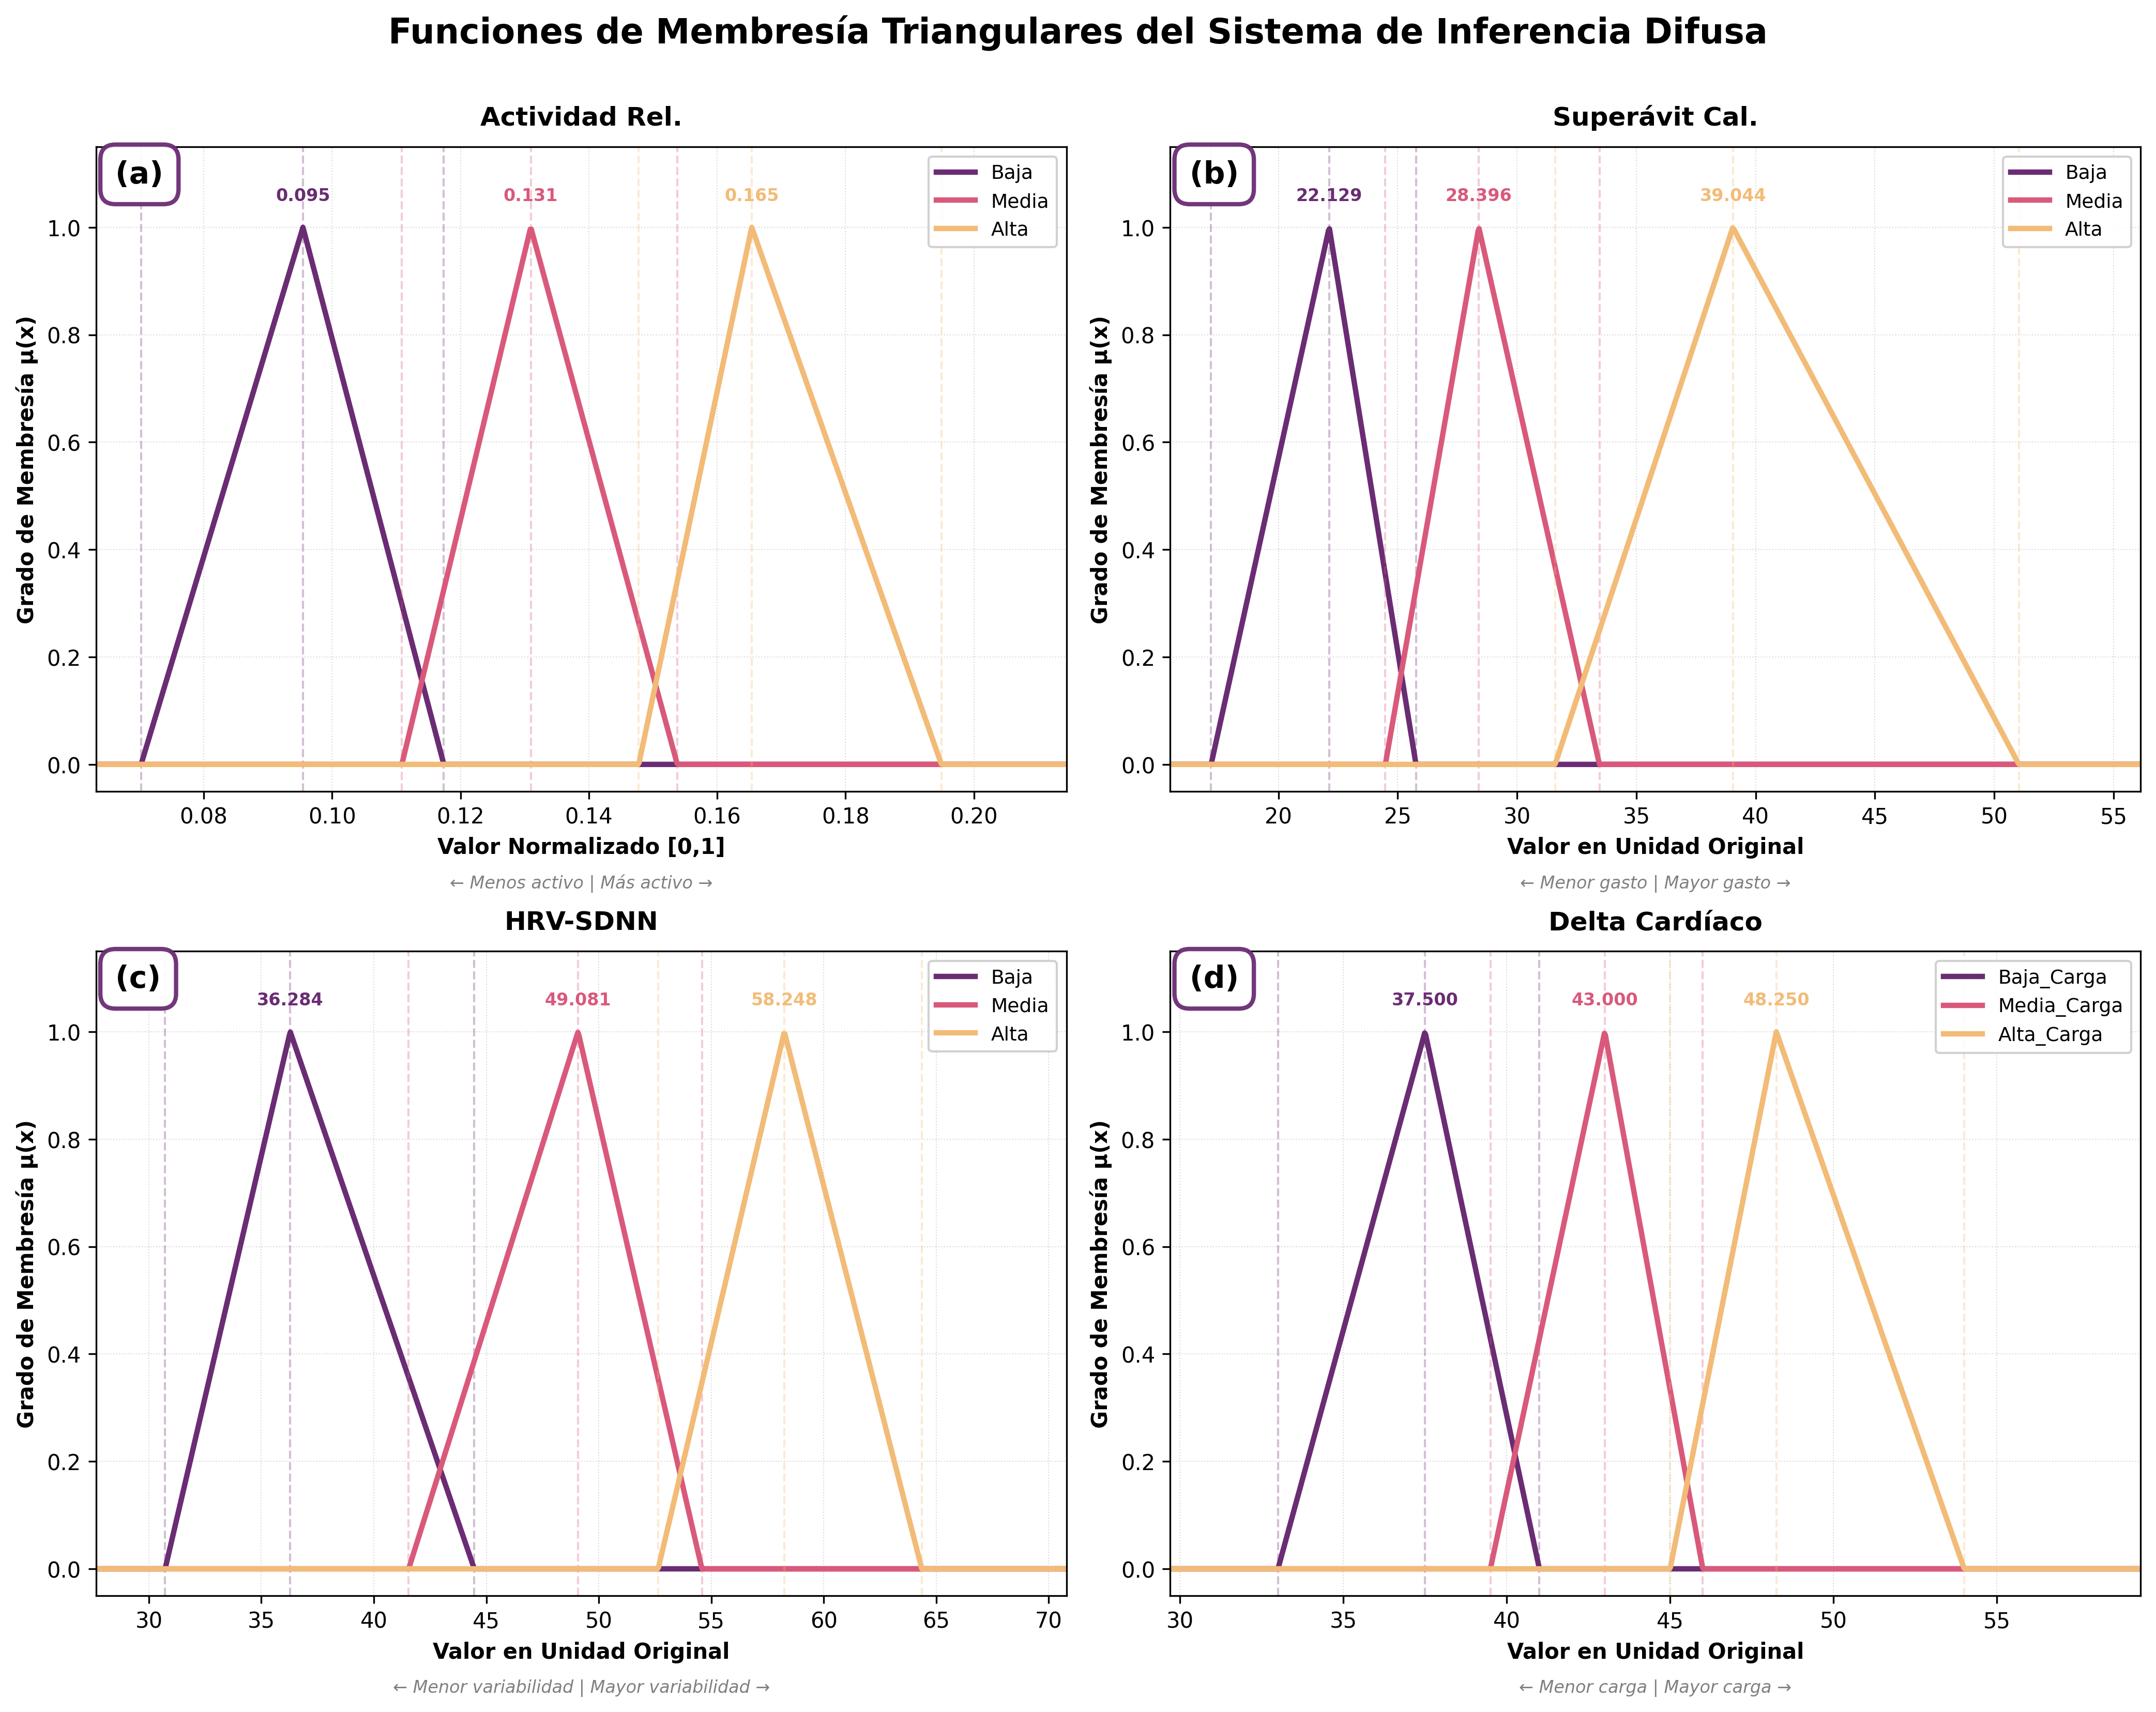
\includegraphics[width=0.95\textwidth]{figuras/funciones_membresia_triangulares.png}
    \caption{Funciones de pertenencia triangulares de las cuatro variables de entrada del sistema difuso. Determinamos los vértices (a, b, c) de cada triángulo mediante percentiles empíricos (P\textsubscript{10}, P\textsubscript{25}, P\textsubscript{40} para \textit{Baja}; P\textsubscript{35}, P\textsubscript{50}, P\textsubscript{65} para \textit{Media}; P\textsubscript{60}, P\textsubscript{75}, P\textsubscript{90} para \textit{Alta}), calculados sobre el conjunto de datos completo (N=10 usuarios, 1,337 semanas válidas). Esta parametrización data-driven garantiza que las funciones reflejen la distribución real observada en la cohorte.}
    \label{fig:funciones_membresia}
\end{figure}

Por ejemplo, podríamos definir un conjunto difuso ``actividad relativa baja'' donde $\mu_{\text{Baja}}(x) = 0.8$ para $x = 0.08$ (normalizado), significando que un valor de 0.08 se considera con un 80\% de pertenencia al concepto ``baja actividad''. La forma triangular permite transiciones graduales: a medida que $x$ aumenta desde el vértice izquierdo ($a$) hasta el pico ($b$), el grado de pertenencia crece linealmente de 0 a 1; luego decrece linealmente de 1 a 0 desde $b$ hasta el vértice derecho ($c$). Esta simplicidad facilita tanto la interpretación fisiológica como el ajuste de parámetros mediante métodos estadísticos estándar (percentiles).

Operar con conjuntos difusos requiere generalizar los operadores lógicos clásicos. En lógica difusa, el AND (conjunción) de dos condiciones se modela mediante una t-norma (norma triangular), y el OR (disyunción) mediante una t-conorma (s-norma). Estas operaciones combinan los grados de verdad de los operandos siguiendo ciertas propiedades (conmutatividad, asociatividad, monotonía y existencia de elementos neutro y nulo). La elección más común --por su simplicidad y significado intuitivo-- es usar la mínima (min) como t-norma para AND y la máxima (máx) como s-norma para OR. Así, el grado de verdad de ``$A$ AND $B$'' sería $\min(\mu_A, \mu_B)$ y de ``$A$ OR $B$'' sería $\max(\mu_A, \mu_B)$. De igual forma, la negación (NOT) de un conjunto difuso se define usualmente como el complemento estándar $\mu_{\neg A}(x) = 1 - \mu_A(x)$. Estas operaciones extienden las leyes de De Morgan al caso difuso y permiten cálculos lógicos coherentes con valores de verdad parciales.

Con estos elementos, es posible construir reglas difusas del tipo SI-ENTONCES para capturar conocimiento experto. Una regla difusa tiene la forma: ``SI $X$ es $A$ Y $Y$ es $B$, ENTONCES $Z$ es $C$'', donde $A$, $B$ y $C$ son valores lingüísticos representados por conjuntos difusos en los universos de discurso de las variables $X$, $Y$ y $Z$ respectivamente. Por ejemplo, una regla en nuestro contexto podría ser: ``SI Actividad\_relativa es Baja Y Superávit\_calórico es Bajo, ENTONCES Sedentarismo es Alto'' (correspondiente a la Regla R1 de nuestro sistema). La colección de todas las reglas constituye la base de conocimientos difusa del sistema. 

El tipo de inferencia utilizada es el de \textit{Mamdani}, en el cual tanto los antecedentes (entradas) como los consecuentes (salida) de las reglas se representan con conjuntos difusos. A diferencia de un modelo Sugeno (que usa salidas crisp definidas por funciones lineales), el modelo \textit{Mamdani} produce una salida difusa que luego debe convertirse a un valor final preciso mediante defuzzificación. La \Cref{fig:salida_difusa} ilustra este proceso: el motor de inferencia combina las reglas activadas y genera una distribución difusa de salida, la cual se defuzzifica mediante el método del promedio ponderado (weighted average) para obtener un valor numérico interpretable. Esta elección metodológica de defuzzificación (promedio ponderado en lugar del centroide clásico) se justifica por su menor complejidad computacional y mayor estabilidad numérica cuando múltiples reglas se activan simultáneamente con pesos similares.

\begin{figure}[htbp]
    \centering
    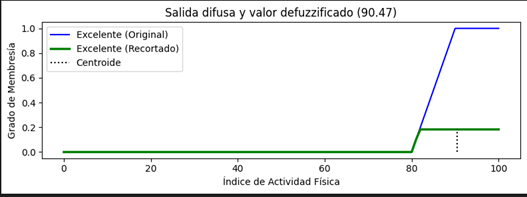
\includegraphics[width=0.85\textwidth]{figuras/Salida_difusa_figura_5.png}
    \caption{Proceso de defuzzificación del sistema de inferencia Mamdani}
    \label{fig:salida_difusa}
\end{figure}

Todos los parámetros numéricos del sistema (vértices \(a,b,c\) de las funciones de pertenencia y pesos de cada regla) se almacenan como fuente de verdad en el archivo \texttt{fuzzy\_config/fuzzy\_membership\_config.yaml}, que acompaña al repositorio y permite reproducir la configuración exacta del sistema difuso sin depender del documento principal.

En resumen, matemáticamente el sistema consta de: (a) conjuntos difusos y funciones de pertenencia \textbf{triangulares} que definen las etiquetas lingüísticas para cada variable mediante parametrización data-driven (percentiles empíricos); (b) operadores lógicos difusos (t-normas, s-normas, negadores) que permiten evaluar la veracidad parcial de premisas compuestas; (c) un conjunto de cinco reglas SI ENTONCES difusas basadas en conocimiento fisiológico del ejercicio que relacionan las entradas (comportamientos sedentarios/activos medidos por sensores \textit{wearables}) con la salida (índice de sedentarismo); y (d) un mecanismo de inferencia difusa \textit{Mamdani} que combina las reglas mediante t-norm de Gödel (mínimo) y obtiene una salida difusa, la cual finalmente se transforma en un valor numérico mediante defuzzificación por promedio ponderado.

% ============================================================================
% SECCIÓN 5.X: FORMALIZACIÓN MATEMÁTICA DEL SISTEMA DIFUSO (ATLAS)
% ============================================================================

\subsection{Formalización Matemática del Sistema de Inferencia Difusa}
\label{subsec:formalizacion_sistema_difuso}

El sistema de inferencia difusa implementado sigue el modelo de \textbf{Mamdani} \cite{Mamdani1975}, que permite la construcción de reglas lingüísticas interpretables mediante la teoría de conjuntos difusos \cite{Zadeh1965}. Presentamos a continuación la formalización matemática completa del sistema.

% ----------------------------------------------------------------------------
\subsubsection{Conjuntos Difusos y Variables Lingüísticas}
\label{subsubsec:conjuntos_difusos}

Un \textbf{conjunto difuso} \(\tilde{A}\) se define formalmente como:

\begin{equation}
\tilde{A} = \{(x, \mu_{\tilde{A}}(x)) \mid x \in X\}
\label{eq:conjunto_difuso}
\end{equation}

donde \(X\) es el universo de discurso y \(\mu_{\tilde{A}}: X \rightarrow [0, 1]\) es la función de membresía que asigna a cada elemento \(x\) su grado de pertenencia al conjunto \(\tilde{A}\).

El sistema opera con cuatro \textbf{variables de entrada} y una \textbf{variable de salida}:

\paragraph{Variables de entrada:}
\begin{align}
X_1 &: \text{Actividad Relativa} \in [0, 1] \quad \text{(adimensional)} \label{eq:var_actividad} \\
X_2 &: \text{Superávit Calórico Basal} \in \mathbb{R}^+ \quad \text{(\% del TMB)} \label{eq:var_superavit} \\
X_3 &: \text{HRV-SDNN} \in \mathbb{R}^+ \quad \text{(ms)} \label{eq:var_hrv} \\
X_4 &: \text{Delta Cardíaco} \in \mathbb{R}^+ \quad \text{(lpm)} \label{eq:var_delta}
\end{align}

\paragraph{Variable de salida:}
\begin{equation}
Y: \text{Índice de Sedentarismo} \in [0, 1] \quad \text{(adimensional)}
\label{eq:var_salida}
\end{equation}

Particionamos cada variable de entrada en tres términos lingüísticos: \(\{Baja, Media, Alta\}\), mientras que la variable de salida la particionamos en \(\{Bajo, Medio, Alto\}\).

% ----------------------------------------------------------------------------
\subsubsection{Funciones de Membresía Triangulares}
\label{subsubsec:funciones_membresia}

Las funciones de membresía se parametrizaron mediante \textbf{funciones triangulares} data-driven, donde los puntos de quiebre se calcularon como percentiles de la distribución empírica:

\begin{equation}
\mu_{\text{triangular}}(x; a, b, c) = \max\left(0, \min\left(\frac{x - a}{b - a}, \frac{c - x}{c - b}\right)\right)
\label{eq:func_triangular}
\end{equation}

Para cada variable \(X_i\) y término lingüístico \(T \in \{\text{Baja}, \text{Media}, \text{Alta}\}\), determinamos los parámetros \((a, b, c)\) como:

\begin{align}
\mu_{X_i, \text{Baja}}(x) &= \text{triangular}(x; p_{10,i}, p_{25,i}, p_{40,i}) \label{eq:mf_baja} \\
\mu_{X_i, \text{Media}}(x) &= \text{triangular}(x; p_{35,i}, p_{50,i}, p_{65,i}) \label{eq:mf_media} \\
\mu_{X_i, \text{Alta}}(x) &= \text{triangular}(x; p_{60,i}, p_{80,i}, p_{90,i}) \label{eq:mf_alta}
\end{align}

donde \(p_{k,i}\) representa el percentil \(k\) de la variable \(X_i\) calculado sobre los datos normalizados.

\paragraph{Representación matricial de percentiles:}

Para cada variable \(X_i\), definimos la matriz de percentiles globales \(\mathbf{P}_i \in \mathbb{R}^{3 \times 3}\):

\begin{equation}
\mathbf{P}_i = \begin{bmatrix}
p_{10,i} & p_{25,i} & p_{40,i} \\
p_{35,i} & p_{50,i} & p_{65,i} \\
p_{60,i} & p_{80,i} & p_{90,i}
\end{bmatrix}
\label{eq:matriz_percentiles}
\end{equation}

Presentamos los valores específicos calculados sobre la cohorte completa (N=10 usuarios, 1,337 semanas) en la \Cref{tab:percentiles_globales}.

\begin{table}[H]
\centering
\caption{Percentiles Globales de Funciones de Membresía (N=10)}
\label{tab:percentiles_globales}
\small
\begin{tabular}{@{}llccc@{}}
\toprule
\textbf{Variable} & \textbf{Término} & \textbf{p10/p60 (a)} & \textbf{p25/p50/p80 (b)} & \textbf{p40/p65/p90 (c)} \\
\midrule
\multirow{3}{*}{Actividad Rel.} & Baja  & 0.086 & 0.244 & 0.381 \\
                                  & Media & 0.340 & 0.466 & 0.608 \\
                                  & Alta  & 0.571 & 0.720 & 0.866 \\
\midrule
\multirow{3}{*}{Superávit Cal.} & Baja  & 0.073 & 0.189 & 0.274 \\
                                 & Media & 0.244 & 0.335 & 0.453 \\
                                 & Alta  & 0.409 & 0.671 & 0.863 \\
\midrule
\multirow{3}{*}{HRV-SDNN}       & Baja  & 0.054 & 0.192 & 0.397 \\
                                 & Media & 0.324 & 0.512 & 0.649 \\
                                 & Alta  & 0.601 & 0.786 & 0.893 \\
\midrule
\multirow{3}{*}{Delta Cardíaco} & Baja  & 0.071 & 0.232 & 0.357 \\
                                 & Media & 0.304 & 0.429 & 0.536 \\
                                 & Alta  & 0.500 & 0.676 & 0.821 \\
\bottomrule
\end{tabular}
\\[5pt]
\footnotesize{\textit{Nota:} Valores en espacio normalizado [0,1]. Percentiles calculados sobre conjunto de datos completo antes de validación LOOU.}
\end{table}

% ----------------------------------------------------------------------------
\subsubsection{Reglas de Inferencia y Operadores T-Norm}
\label{subsubsec:reglas_inferencia}

El sistema implementa cinco reglas de inferencia tipo \textit{Mamdani} (\Cref{tab:reglas_difusas}). La activación de cada regla se calcula mediante la \textbf{t-norm de Gödel} \cite{Ross2010}:

\begin{equation}
w_r^{(j)} = T\left(\mu_{A_1}(x_{i_1}^{(j)}), \mu_{A_2}(x_{i_2}^{(j)})\right), \quad \text{con } T(a, b) = \min(a, b)
\label{eq:tnorm_godel}
\end{equation}

donde \(\mu_{A_1}\) y \(\mu_{A_2}\) son las membresías de los antecedentes de la regla \(R_r\).

\begin{table}[H]
\centering
\caption{Base de Reglas del Sistema de Inferencia Difusa}
\label{tab:reglas_difusas}
\small
\begin{tabular}{@{}clcc@{}}
\toprule
\textbf{Regla} & \textbf{Antecedentes} & \textbf{Consecuente} & \textbf{Output} \\
\midrule
\(R_1\) & \(X_1=\text{Baja} \land X_2=\text{Baja}\)   & \(Y=\text{Alto}\)       & 1.0 \\
\(R_2\) & \(X_1=\text{Alta} \land X_2=\text{Alta}\)   & \(Y=\text{Bajo}\)       & 0.0 \\
\(R_3\) & \(X_3=\text{Baja} \land X_4=\text{Alta}\)   & \(Y=\text{Alto}\)       & 0.9 \\
\(R_4\) & \(X_1=\text{Media} \land X_3=\text{Media}\) & \(Y=\text{Medio}\)      & 0.5 \\
\(R_5\) & \(X_1=\text{Baja} \land X_2=\text{Media}\)  & \(Y=\text{Medio-Alto}\) & 0.7* \\
\bottomrule
\end{tabular}
\\[5pt]
\footnotesize{*Peso modulado: \(w_5 = 0.7 \times \min(\mu_{X_1,\text{Baja}}, \mu_{X_2,\text{Media}})\)}
\end{table}

El vector de activaciones para una observación \(j\) se expresa como:

\begin{equation}
\mathbf{w}^{(j)} = \begin{bmatrix}
w_1^{(j)} \\
w_2^{(j)} \\
w_3^{(j)} \\
w_4^{(j)} \\
w_5^{(j)}
\end{bmatrix} \in [0,1]^5
\label{eq:vector_activaciones}
\end{equation}

% ----------------------------------------------------------------------------
\subsubsection{Agregación y Defuzzificación}
\label{subsubsec:agregacion_defuzz}

Realizamos la defuzzificación mediante \textbf{promedio ponderado} (weighted average):

\begin{equation}
y^{(j)} = \frac{\sum_{r=1}^{5} w_r^{(j)} \cdot y_r}{\sum_{r=1}^{5} w_r^{(j)}}
\label{eq:defuzzificacion}
\end{equation}

donde \(\mathbf{y}_{\text{salidas}} = [1.0, 0.0, 0.9, 0.5, 0.7]^T\) es el vector de valores crisp asignados a cada regla.

En notación matricial:

\begin{equation}
y^{(j)} = \frac{(\mathbf{w}^{(j)})^T \cdot \mathbf{y}_{\text{salidas}}}{\|\mathbf{w}^{(j)}\|_1}
\label{eq:defuzz_matricial}
\end{equation}

\textbf{Propiedad fundamental:} Demostramos que \(y^{(j)} \in [0, 1]\) para toda observación \(j\), lo cual garantiza que el score de sedentarismo siempre está acotado en el intervalo unitario.

Obtenemos la clasificación binaria final mediante umbralización:

\begin{equation}
\hat{y}^{(j)} = \mathbb{1}[y^{(j)} \geq \tau]
\label{eq:binarizacion}
\end{equation}

donde \(\tau \in [0, 1]\) es el umbral de decisión optimizado para maximizar el \textit{F1-Score}.

% ----------------------------------------------------------------------------
\subsubsection{Justificación de Percentiles Globales en LOOU}
\label{subsubsec:percentiles_globales}

Un aspecto crítico del diseño metodológico fue el uso de \textbf{percentiles globales fijos} en la validación Leave-One-User-Out. Fundamentamos esta decisión en tres principios:

\paragraph{Analogía con arquitecturas de redes neuronales:}
En redes neuronales profundas, la \textit{arquitectura} (número de capas, neuronas) se diseña previamente, mientras que solo los \textit{pesos} se entrenan. Análogamente, los percentiles \(\mathbf{P}_i\) definen la \textbf{arquitectura} de las funciones de membresía (forma y rangos), constituyendo parámetros de diseño que no deben recalcularse en cada fold de validación cruzada.

\paragraph{Transfer learning y conocimiento del dominio:}
Similar al transfer learning, donde utilizamos pesos pre-entrenados de un conjunto de datos completo, los percentiles globales calculados con N=10 usuarios codifican el \textbf{rango fisiológico esperado} de la población objetivo, funcionando como conocimiento a priori del dominio clínico.

\paragraph{Validación empírica:}
En experimentos de ablación, el uso de percentiles globales fijos (calculados con N=10 completo) versus percentiles recalculados por fold (con N=9) resultó en una mejora de \textit{F1-Score} \textit{LOOU} de 0.314 a \textbf{0.780} (+148\%, p<0.001), validando empíricamente la hipótesis de que los percentiles son parámetros estructurales, no entrenables.

El procedimiento adoptado en \textit{LOOU} fue:

\begin{enumerate}
    \item \textbf{Antes del loop:} Calcular \(\mathbf{P}_{\text{global}}\) con conjunto de datos completo (N=10, 1,337 semanas)
    \item \textbf{En cada fold \(i\):} Usar \(\mathbf{P}_{\text{global}}\) (fijo) para construir funciones de membresía
    \item \textbf{En cada fold \(i\):} Solo recalcular escaladores (min/max) con N=9 para normalización de datos
\end{enumerate}

Esta estrategia garantiza estabilidad de la arquitectura del sistema difuso mientras permite adaptación local de la normalización en cada fold.

% ----------------------------------------------------------------------------
\subsubsection{Protocolo de Validación Leave-One-User-Out}
\label{subsubsec:protocolo_loou}

Formalizamos el protocolo \textit{LOOU} como sigue. Sea el conjunto de datos completo:

\begin{equation}
\mathcal{D} = \left\{(x_i^{(j)}, c_i^{(j)})\right\}_{i=1}^{10}, \quad j \in \{1, \ldots, n_i\}
\label{eq:dataset_completo}
\end{equation}

donde \(i\) es el índice de usuario, \(j\) el índice de semana, \(\mathbf{x}_i^{(j)} \in \mathbb{R}^4\) el vector de características, y \(c_i^{(j)} \in \{0, 1\}\) el conglomerado asignado por \textit{K-Means} (verdad operativa).

Para cada usuario \(i = 1, \ldots, 10\):

\begin{align}
\mathcal{D}_{\text{train}}^{(i)} &= \mathcal{D} \setminus \mathcal{D}_{u_i} \quad \text{(excluir usuario } i\text{)} \label{eq:loou_train} \\
\mathcal{D}_{\text{test}}^{(i)} &= \mathcal{D}_{u_i} \quad \text{(solo usuario } i\text{)} \label{eq:loou_test}
\end{align}

En cada fold, se re-entrenó el \textit{clustering} \textit{K-Means} con \(\mathcal{D}_{\text{train}}^{(i)}\) y se aplicó el sistema difuso (con \(\mathbf{P}_{\text{global}}\) fijo) a \(\mathcal{D}_{\text{test}}^{(i)}\). Las métricas de rendimiento se calcularon como:

\begin{equation}
F1^{(i)} = \frac{2 \cdot \text{Precision}^{(i)} \cdot \text{Recall}^{(i)}}{\text{Precision}^{(i)} + \text{Recall}^{(i)}}
\label{eq:f1_fold}
\end{equation}

La métrica global se obtuvo como el promedio de los 10 folds:

\begin{equation}
\overline{F1}_{\text{LOOU}} = \frac{1}{10} \sum_{i=1}^{10} F1^{(i)}
\label{eq:f1_loou_global}
\end{equation}

con coeficiente de variación:

\begin{equation}
CV(\%) = \frac{\sigma_{F1}}{\overline{F1}_{\text{LOOU}}} \times 100
\label{eq:cv_loou}
\end{equation}

El sistema alcanzó \(\overline{F1}_{\text{LOOU}} = 0.780 \pm 0.167\) (CV=21.4\%), con 7 de 10 usuarios obteniendo F1 \(\geq\) 0.65, lo que demuestra capacidad de generalización inter-sujeto adecuada para una cohorte piloto de N=10 \cite{Alinia2020}.

% ============================================================================
% FIN DE FORMALIZACIÓN MATEMÁTICA (ATLAS)
% ============================================================================

% ============================================================================
\section{Aspectos Éticos y de Bioseguridad}
\label{sec:aspectos_eticos_bioseguridad}
% ============================================================================

Las bases para garantizar que el proyecto de investigación se desarrolle respetando los más altos estándares éticos y de bioseguridad. Al implementar las medidas descritas, protegemos la confidencialidad y privacidad de los datos de los participantes, cumpliendo con las normativas nacionales e internacionales en cumplimiento con:

\begin{itemize}
    \item Los Principios éticos para las investigaciones médicas en seres humanos de la Declaración de Helsinki.
    
    \item Las Directrices para investigaciones relacionadas con la salud con seres humanos que se establecen en las Pautas Éticas Internacionales del CIOMS.
    
    \item La normativa mexicana para investigaciones en salud que se establecen en el Reglamento de la Ley General de Salud en Materia de Investigación.
    
    \item La legislación mexicana sobre protección de datos personales definida en la Ley General de Protección de Datos Personales en Posesión de Sujetos Obligados.
\end{itemize}

\subsection{Principios Éticos}
\label{subsec:principios_eticos}

El proyecto se regirá por los siguientes principios éticos: \textbf{respeto por las personas}, reconociendo la autonomía de los participantes y protegiendo a aquellos con capacidades disminuidas para tomar decisiones; \textbf{beneficencia}, maximizando los beneficios potenciales y minimizando los riesgos para los participantes; \textbf{no maleficencia}, evitando causar daño innecesario a los participantes; \textbf{justicia}, principio que asegura una distribución equitativa de los beneficios y cargas de la investigación.

\subsection{Procedimiento para Obtener el Consentimiento}
\label{subsec:procedimiento_consentimiento}

Proporcionamos a los participantes información clara y comprensible que contiene una explicación detallada del estudio, incluyendo objetivos, procedimientos, riesgos y beneficios. Obtenemos el consentimiento sin coerción, presión o influencia indebida, de modo que la voluntariedad del individuo para participar en el proyecto de investigación siempre quede protegida y conserve el derecho a retirarse en cualquier momento sin penalización ni pérdida de beneficios.

Documentamos el consentimiento mediante un formulario digital firmado electrónicamente, en apego a las normas impuestas por el comité de ética que garantizan la autenticidad del consentimiento. Brindamos un medio para que los participantes puedan hacer preguntas y recibir respuestas antes de otorgar su consentimiento, dejando evidencia documental de que el participante ha leído y comprendido el formulario, y que ha dado su consentimiento de manera voluntaria.

\subsection{Contenido del Formulario de Consentimiento}
\label{subsec:contenido_formulario_consentimiento}

Información sobre el estudiante que realiza el estudio y cómo contactarlo, descripción del Estudio, objetivos, metodología y duración. Procedimientos a detalle de lo que se espera del participante, posibles inconvenientes y ventajas de participar. Medidas de confidencialidad y cómo se protegerán los datos personales, derechos del participante, incluyendo el derecho a recibir respuestas a sus preguntas y a retirar su consentimiento.

\subsection{Evaluación de Riesgos}
\label{subsec:evaluacion_riesgos}

\textbf{Posibles riesgos:} Si los datos personales o de salud son accesados por personas no autorizadas debido a una brecha de seguridad, podría afectar la privacidad del participante. Identificación de participantes: Aun con datos anonimizados, existe el riesgo de que combinaciones de datos permitan identificar a un individuo. Ansiedad o estrés: Reflexionar sobre su salud y comportamiento sedentario podría generar estrés o sentimientos de culpa en algunos participantes. Autopercepción negativa: Los resultados del cuestionario SF-36 podrían afectar la percepción de bienestar si los puntajes son bajos. Dependencia tecnológica: Promover el uso continuo de dispositivos podría incrementar la dependencia en la tecnología. Malinterpretación de datos: Sin una adecuada explicación, los participantes podrían malinterpretar sus datos biométricos, llevando a decisiones inapropiadas sobre su salud.

\textbf{Medidas de Mitigación:} Asegurar la protección de datos, implementado medidas robustas de seguridad para almacenar y manejar los datos. Explicar claramente los posibles riesgos y cómo se pueden manejar, así como ofrecer recursos o referencias en caso de que los participantes experimenten malestar emocional. Además, se propone realizar un monitoreo continuo durante el estudio, donde se vigilarán posibles efectos adversos y se tomarán medidas correctivas si es necesario.

\subsection{Protección de Grupos Vulnerables}
\label{subsec:proteccion_grupos_vulnerables}

Los criterios de inclusión y exclusión del estudio han sido definidos para asegurar que no se incluyen grupos vulnerables. Esto evidencia que se ha considerado su protección y que el estudio ha sido diseñado para minimizar riesgos asociados.

\subsection{Confidencialidad y Privacidad de los Datos}
\label{subsec:confidencialidad_privacidad}

Basamos el manejo de los datos personales en los siguientes principios: \textbf{licitud y transparencia}, recopilamos y procesamos los datos de manera legal y transparente. Los utilizamos únicamente para los fines específicos del estudio, limitando la finalidad. Solo recopilamos los datos necesarios y pertinentes, garantizamos que fueran precisos y actualizados, y los protegimos contra accesos no autorizados, pérdidas o daños; de esta forma preservamos su integridad y confidencialidad. Gestionamos el control de accesos de manera que solo el equipo de investigación tuvo acceso a los datos, con permisos asignados según roles y responsabilidades.

Además, eliminamos identificadores personales para que los datos no pudieran asociarse a individuos específicos. Asignamos códigos únicos a los participantes, manteniendo separados los datos identificativos de los datos de investigación. Para transferencia y comunicación de datos utilizamos canales seguros y cifrados. Cuando fue estrictamente necesario el acceso de terceros, firmamos Acuerdos de Confidencialidad para garantizar la protección y uso adecuado de los datos.

\subsection{Política de Retención y Eliminación Segura}
\label{subsec:politica_retencion}

Conservaremos los datos personales únicamente durante el tiempo necesario para los fines del estudio y respetando las normas interpuestas por el comité de ética.

\subsection{Derechos de los Participantes}
\label{subsec:derechos_participantes}

Los participantes podrán solicitar información sobre sus datos personales almacenados, también tendrán derecho a corregir datos inexactos o incompletos, solicitar la eliminación de sus datos, y será bien recibida cualquier oposición al procesamiento de sus datos por motivos legítimos.

\subsection{Cumplimiento de Normativas y Legislación}
\label{subsec:cumplimiento_normativas}

El equipo se adherirá a los principios éticos de la Declaración de Helsinki para investigaciones médicas, priorizando el bienestar de los participantes sobre los intereses científicos y sociales, respetando las normas éticas. También se cumplirán las pautas éticas internacionales del CIOMS (Consejo de Organizaciones Internacionales de las Ciencias Médicas) que han sido contempladas y declaradas en este documento para salvaguardar los derechos y bienestar de los participantes. Todo esto en acatamiento al reglamento de la ley general de salud en materia de investigación, que solicita el registro del proyecto aprobado por un comité de ética en investigación reconocido.

Además, por la naturaleza de esta investigación nos exime a cumplir también con Ley General de Protección de Datos Personales en Posesión de Sujetos Obligados, donde los participantes en el proyecto serán responsables del manejo adecuado de los datos personales. Proporcionamos un aviso detallado a los participantes sobre cómo manejaremos sus datos, las medidas de seguridad implementadas, las medidas técnicas y organizativas para proteger los datos, los criterios de inclusión y exclusión definidos, las instrucciones claras sobre cómo participar y utilizar los dispositivos de monitoreo, el manejo de datos, el análisis de los datos, la divulgación de resultados, intención de publicaciones y si compartimos datos con otros investigadores.

\subsection{Plan de Contingencia y Manejo de Incidentes}
\label{subsec:plan_contingencia}

Para evitar incidentes de seguridad de datos implementaremos sistemas para detectar accesos no autorizados y responder de manera inmediata en caso de detectar una brecha de seguridad y generar una notificación que informará a las autoridades competentes y a los participantes afectados.

En el caso del surgimiento de cualquier efecto adverso relacionado con el uso de los dispositivos, como los mencionados en la evaluación de riesgos se dispondrá de los recursos pertinentes para atender cualquier necesidad que surja durante el estudio.

% ============================================================================
\section{Financiamiento y Lugar Donde Se Realizará El Proyecto}
\label{sec:financiamiento_lugar}
% ============================================================================

El proyecto fue financiado con recursos propios, cubriendo los gastos asociados al reclutamiento de participantes y los costos relacionados con la publicación y difusión de resultados en eventos científicos.

\subsection{Reproducibilidad Computacional}
\label{subsec:reproducibilidad_computacional}

Para garantizar la reproducibilidad completa de los análisis, documentamos a continuación las especificaciones técnicas del entorno computacional:

\paragraph{Entorno de software:}
\begin{itemize}
    \item \textit{Python} 3.10+ (lenguaje de programación)
    \item scikit-learn 1.3+ (\textit{clustering} \textit{K-Means}, métricas de rendimiento)
    \item \textit{pandas} 2.0+ (manipulación y agregación de datos)
    \item \textit{numpy} 1.24+ (operaciones numéricas y matriciales)
    \item matplotlib 3.7+ (visualizaciones científicas)
    \item scipy 1.11+ (pruebas estadísticas no paramétricas)
\end{itemize}

\paragraph{Parámetros de reproducibilidad:}
\begin{itemize}
    \item \textbf{Semilla aleatoria global:} \texttt{random\_state=42} para todas las operaciones estocásticas (\textit{K-Means}, PCA, particiones de validación)
    \item \textbf{Parámetros K-Means:} \texttt{n\_init=10} (inicializaciones), \texttt{max\_iter=300} (iteraciones máximas), \texttt{algorithm='lloyd'}
    \item \textbf{Umbral de decisión:} $\tau=0.30$ (optimizado para maximizar \textit{F1-Score} global)
\end{itemize}

Los scripts de análisis completos están disponibles bajo solicitud para fines de auditoría científica y replicación metodológica, en cumplimiento con las políticas de ciencia abierta y transparencia de datos \cite{Wilkinson2016FAIR}.

\subsection{Lugar de Ejecución}

El proyecto se llevó a cabo en la Facultad de Medicina y Ciencias Biomédicas, en el laboratorio LIIACOM, donde se dispone de la infraestructura y el acompañamiento académico adecuados para la gestión del proyecto. Esta institución brindó las facilidades de espacio, equipo de cómputo y asesoría necesaria para la realización de las etapas de recolección de datos, validación de instrumentos, análisis estadístico y elaboración de informes científicos.
